%!TeX spellcheck = fr-FR
\documentclass[10pt,fleqn]{article} % Default font size and left-justified equations
\usepackage[%
    pdftitle={SLCI : Transformée de Laplace},
    pdfauthor={Xavier Pessoles}]{hyperref}

\usepackage{import}
\usepackage{subcaption}
\subimport{../../../../style/}{preambule.tex}
%\fichetrue
\fichefalse
\proftrue
%\proffalse
%\tdtrue
\tdfalse
\courstrue
%\coursfalse
\subimport{../../../../style/}{new_style}
\subimport{../../../../style/}{macros_SII}
\subimport{../../../../style/}{preambule_trou.tex}

\usepackage{siunitx}
% -------------------------------------
% Déclaration des titres
% -------------------------------------

\def\discipline{Enseignement \\Technologique \\ Transversal}
\def\xxtete{Enseignement Technologique Transversal}

\def\classe{1 STI2D}
\def\xxnumpartie{Seq 3}
\def\xxpartie{Alimenter un système en énergie}

\def\xxnumchapitre{Séance 3}
\def\xxchapitre{\hspace{.12cm} Convertir l'énergie}

\def\xxposongletx{2}
\def\xxposonglettext{1.45}
\def\xxposonglety{23}
\def\xxonglet{Seq. 3 -- Se. 3}

\def\xxactivite{Cours}
\def\xxauteur{\textsl{Geoffrey Vaquette}}

\def\xxcompetences{%
\textsl{%
\textbf{Prérequis :}
\begin{itemize}[label=\ding{112},font=\color{ocre}]
\item Analyse fonctionnelle de la chaîne d'énergie
\end{itemize}
\textbf{Savoirs et compétences :}
\begin{itemize}[label=\ding{112},font=\color{ocre}]
\item CO2.1	Identifier les flux et la forme de l'énergie, caractériser ses transformations et/ou modulations et estimer l'efficacité globale d'un système.
\end{itemize}
%
}}

\def\xxfigures{
\begin{center}
% 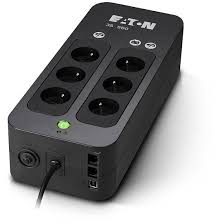
\includegraphics[width=2cm]{images/onduleur} \\
% 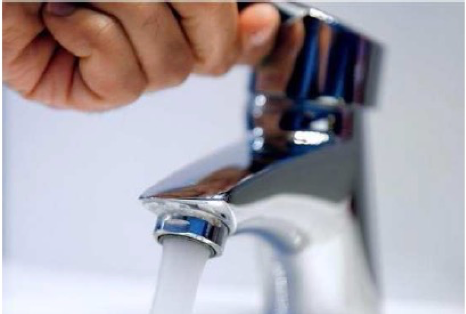
\includegraphics[width=2cm]{images/robinet} \\
%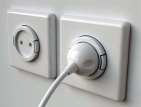
\includegraphics[width=2cm]{images/prise.png} \\
\end{center}
}%figues de la page de garde
\def\xxpied{%
Convertir de l'énergie \xxactivite%
}

%---------------------------------------------------------------------------

\renewcommand{\RemplirTrou}{false}
\begin{document}
\chapterimage{images/bandeau}
\subimport{../../../../style/}{new_pagegarde}

\begin{figure}[h]
  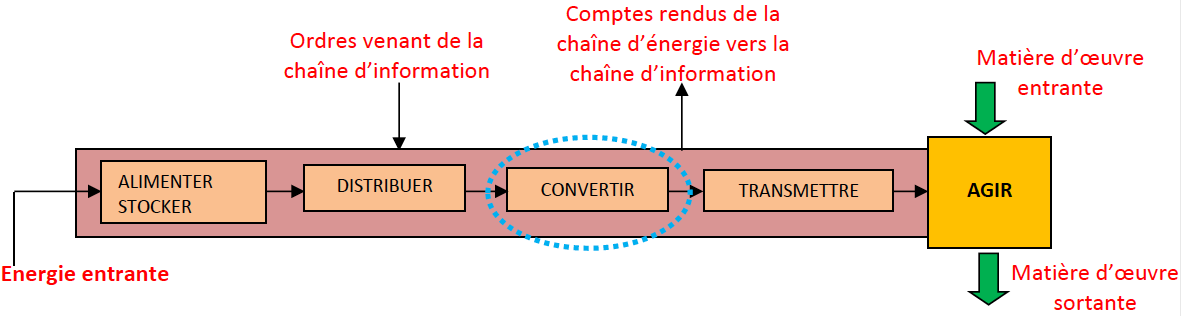
\includegraphics[width=\textwidth]{images/S03_C03}
  \caption{La fonction « Convertir » dans la chaîne d'énergie}
  \label{fig:chaine}
\end{figure}

Une fois que le système est alimenté en énergie et que celle-ci est distribuée, il est parfois (souvent) nécessaire de convertir cette énergie d’entrée pour que le système remplisse sa fonction d’usage.
La fonction « Convertir » permet cette transformation d’énergie.

\begin{obj}
  Identifier quels sont les éléments assurant la fonction « Convertir » de la chaîne d’énergie d’un système.
\end{obj}

\section{Généralités sur les convertisseurs (ou actionneurs)}
\begin{definition}
  Les composants réalisant la conversion d’énergie sont appelés « actionneurs » : ils permettent de convertir l'énergie reçue en travail utile pour exécuter les tâches du système.
\end{definition}


Un actionneur est caractérisé par :
\begin{itemize}
  \item Son énergie en entrée (Énergie avant transformation)
  \begin{itemize}
    \item hydraulique
    \item pneumatique
    \item électrique
    \item mécanique
    \item combustible
    \item solaire
    \item musculaire
    \item \dots
  \end{itemize}
  \item Son énergie en sortie (énergie après transformation)
  \begin{itemize}
    \item hydraulique
    \item électrique
    \item mécanique
    \item combustible
    \item lumineuse
    \item \dots
  \end{itemize}



\end{itemize}
\pagebreak
\section{Exemples d'actionneurs}

\begin{figure}[h]
  \centering
  \begin{subfigure}{0.25\textwidth}
    \centering
    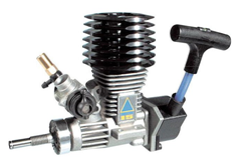
\includegraphics[width=0.9\textwidth,height=.1\textheight,keepaspectratio]{images/moteur_thermique}
    \caption{Moteur thermique}
  \end{subfigure}\hfill
  \begin{subfigure}{.25\textwidth}
    \centering
    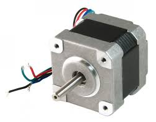
\includegraphics[width=0.9\textwidth,height=.1\textheight,keepaspectratio]{images/moteur_paspas}
    \caption{Moteur }
  \end{subfigure}\hfill
  \begin{subfigure}{0.25\textwidth}
    \centering
    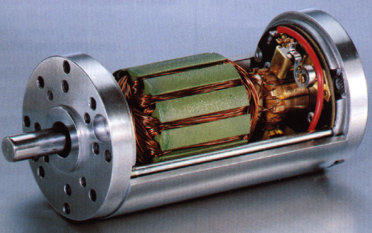
\includegraphics[width=0.9\textwidth,height=.1\textheight,keepaspectratio]{images/moteur_continu}
    \caption{Moteur électrique}
  \end{subfigure}\hfill
  \begin{subfigure}{.25\textwidth}
    \centering
    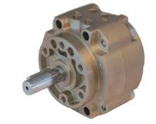
\includegraphics[width=0.9\textwidth,height=.1\textheight,keepaspectratio]{images/verin_rotatif}
    \caption{Vérin rotatif}
  \end{subfigure}\\
  \begin{subfigure}{0.25\textwidth}
    \centering
    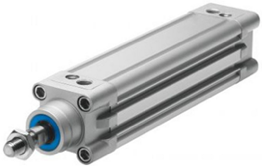
\includegraphics[width=0.9\textwidth,height=.1\textheight,keepaspectratio]{images/verin_pneu}
    \caption{Vérin pneumatique}
  \end{subfigure}\hfill
  \begin{subfigure}{.25\textwidth}
    \centering
    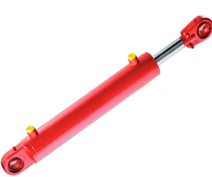
\includegraphics[width=0.9\textwidth,height=.1\textheight,keepaspectratio]{images/verin_hydrqu}
    \caption{Vérin hydraulique}
  \end{subfigure}
  \begin{subfigure}{0.25\textwidth}
    \centering
    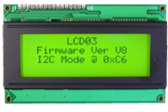
\includegraphics[width=0.9\textwidth,height=.1\textheight,keepaspectratio]{images/afficheur}
    \caption{Afficheur}
  \end{subfigure}\hfill
  \begin{subfigure}{.24\textwidth}
    \centering
    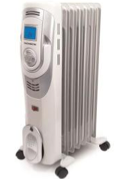
\includegraphics[width=0.9\textwidth,height=.1\textheight,keepaspectratio]{images/radiateur}
    \caption{Radiateur}
  \end{subfigure}
  \caption{Quelques exemples d'actionneurs}
  \label{fig:exemples}
\end{figure}

\subsection{Fonctionnement d'un chauffage simple}

Un chauffage simple (radiateur) peut être assimilé à une résistance. La chaleur est créée à partir de l'énergie électrique par \textbf{effet joule} :

Lorsque les électrons se déplacent dans un conducteur, interagissent avec les atomes constitutifs de la matière. Cette interaction résiste à leur déplacement et crée de la chaleur.

\begin{aretenir}
  La puissance thermique dissipée par effet joule dans une résistance est égale à la puissance électrique qui traverse cette résistance.
\end{aretenir}

\subsection{Fonctionnement d'un vérin}
Qu'il soit pneumatique ou hydraulique, un verin crée un mouvement à partir de la pression du fluide qui l'actionne. Dans le cas d'un vérin pneumatique, le fluide est sous forme d'air comprimé. Dans le cas d'un vérin hydraulique, il s'agit le plus souvent d'huile sous pression.

Il existe deux types de vérins :
\begin{itemize}
  \item Simple effet : Les vérins « simple effet » n'ont qu'\textbf{une direction de travail}. Cela signifie qu'ils ne forcent que dans un sens. La tige du vérin est ramenée par un ressort.
  \item Double effets : Les vérins « double effet » ont \textbf{deux directions de travail}. Cela signifie qu'ils peuvent forcer dans les deux sens. Le fluide sous pression peut arriver d'un côté ou de l'autre du vérin pour faire rentrer ou sortir la tige selon l'effet désiré.
\end{itemize}

\begin{figure}[h]
  \centering
  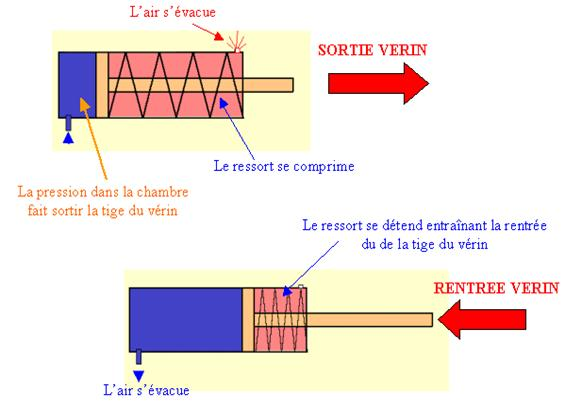
\includegraphics[height=.2\textheight]{images/verin}
  \caption{Principe de fonctionnement d'un vérin simple effet}
  \label{fig:verin_simple}
\end{figure}

Dans le cas d'un vérin simple effet (Figure~\ref{fig:verin_simple}), lorsque le fluide arrive sous pression, il pousse la tige du vérin. Cette force a pour effet de mettre en mouvement le vérin. Lorsque le fluide n'est plus sous pression, le ressort poursse le vérin dans l'autre sens.



\subsection{Fonctionnement d'un moteur électrique}
Les moteurs électriques fonctionnent par un phénomème électromagnétique. Comme représenté sur la Figure~\ref{fig:induction}, lorsqu'une inductance (bobine de fil) est parcourue par un courant électrique, elle se comporte comme un aimant.

\begin{remark}
    Pour connaître le sens du flux magnétique créé par une bobine, on utilise la règle du tire-bouchon : on imagine un tire-bouchon tournant dans le sens du courant ; le nord est du côté vers lequel avance ce tire-bouchon imaginaire.
\end{remark}


\begin{figure}[h]
  \centering
  \begin{subfigure}{0.5\textwidth}
    \centering
    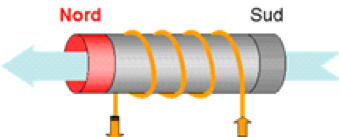
\includegraphics[width=0.5\textwidth]{images/indu_aimant1}
    % \caption{}
  \end{subfigure}\hfill
  \begin{subfigure}{.5\textwidth}
    \centering
    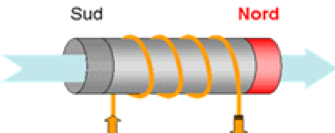
\includegraphics[width=0.5\textwidth]{images/indu_aimant2}
    % \caption{Symbole électrique d'un transistor}
  \end{subfigure}
  \caption{Un courant dans une bobine induit un champs magnétique}
  \label{fig:induction}
\end{figure}
Un moteur électrique est un composant exploitant l'interaction entre des aimants et le courant pour créer un mouvement à partir d'électricité (force électro-magnétique).

\begin{aretenir}
  Les moteurs électriques sont tous constitués d'un \textbf{stator} fixe par rapport auquel un \textbf{rotor} tourne.
\end{aretenir}


\begin{obj}
  Un moteur électrique doit sans cesse faire varier le champs magnétique pour permettre la mise en rotation du rotor. Dit autrement, un moteur électrique ré-oriente sans cesse les «aimants» qu'il génère, afin de faire l'axe.
\end{obj}

\subsubsection{Moteur à courant continu}
\begin{figure}[h]
  \centering
  \begin{subfigure}{0.5\textwidth}
    \centering
    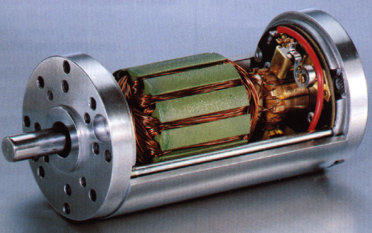
\includegraphics[width=0.7\textwidth]{images/moteur_continu}
    \caption{Vue démonté}
  \end{subfigure}\hfill
  \begin{subfigure}{.5\textwidth}
    \centering
    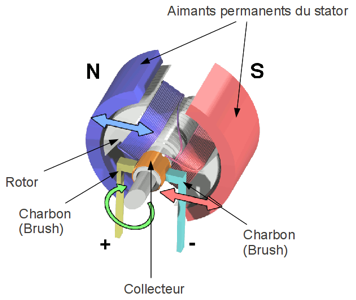
\includegraphics[width=0.7\textwidth]{images/moteur_continu_explose}
    \caption{Schéma de principe}
  \end{subfigure}
  \caption{Moteur à courant continu}
  \label{fig:induction}
\end{figure}

Dans un moteur à courant continu, le stator est composé d'aimants permanents. Ces aimants créent un champs magnétique fixe (puisqu'ils ne bougent pas).
Le rotor est quant à lui composé de bobines électriques qui, parcourues par un courant continu, se comportent comme des aimants.

Afin de changer le sens du champs magnétique, le \textbf{rotor} est alimenté par un système de balais et de collecteurs.

\begin{aretenir}
  Le courant continu injecté via les balais au collecteur, traverse le bobinage du rotor et change de sens pendant la rotation grâce au système balais/collecteur, ainsi le bobinage est toujours de polarité opposée aux aimants fixes ce qui entraîne le mouvement de rotation
\end{aretenir}

\subsubsection{Moteurs à courant alternatif (synchrones et asynchornes)}

\begin{figure}
  \centering
  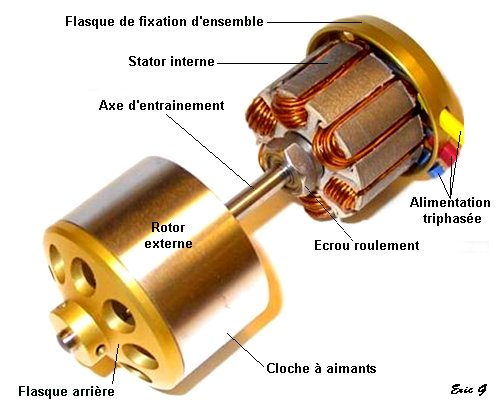
\includegraphics[width=0.3\textwidth]{images/moteur11}
  \caption{Moteur alternatif}
  \label{fig:mot}
\end{figure}

Alimentées par un (des) courant(s) alternatif(s) sinusoïdaux, ce type de moteur utilise la variation du courant pour créer un champs magnétique tournant.

Dans le cas de moteurs triphasés (les plus courants), le \textbf{stator} est composé d'au moins trois bobines (paires de pôles) permettant la génération d'un champs magnétique tournant.

Les deux types de moteurs (synchrones et asynchornes) se différencient principalement par la structure de leur rotor :
\paragraph{Les moteurs synchrones}
Le \textbf{rotor} est composé d'un aimant permanent (ou d'un électroaimant) qui va suivre le champs magnétique créé par le stator.

\begin{aretenir}
  Le rotor des moteurs synchrones tournent à la même vitesse que le champs créé par le stator. Puisque ce champs est créé par un courant alternatif, c'est la fréquence de ce courant qui dicte la vitesse de rotation du moteur.
\end{aretenir}

\begin{warn}
  Pour démarer un moteur synchrone, il est souvent indispensable de faire varier sa fréquence d'alimentation.
\end{warn}

\paragraph{Les moteurs asynchrones}
Le \textbf{rotor} est constitué de barre d’aluminium (cage d’écureuil) : le rotor tourne dans le même sens que le champ magnétique mais pas à la même vitesse. C'est pourquoi ces moteurs sont appelés moteurs asynchrones.

\begin{figure}[h]
  \centering
  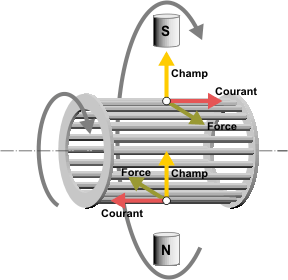
\includegraphics[width=.3\textwidth]{images/moteur-asynchrone}
  \caption{Cage d'écureuil}
  \label{fig:ecu}
\end{figure}
\pagebreak
\subsubsection{Moteur pas à pas}
Dans un moteur pas à pas, on active les bobines de façon à orienter le rotor dans l'axe voulu. Il permet d'obtenir un asservissement en position de l'axe (on peut choisir facilement l'orientation de l'axe).
\begin{figure}[h]
  \centering
  \begin{subfigure}{0.245\textwidth}
    \centering
    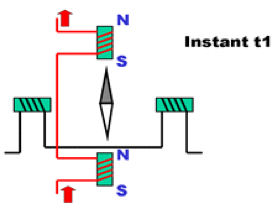
\includegraphics[width=0.9\textwidth]{images/moteur_paspas1}
    \caption{Instant $t_1$}
  \end{subfigure}
  \begin{subfigure}{.245\textwidth}
    \centering
    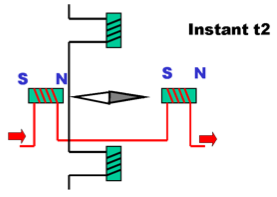
\includegraphics[width=0.9\textwidth]{images/moteur_paspas2}
    \caption{Instant $t_2$}
  \end{subfigure}
  \begin{subfigure}{0.245\textwidth}
    \centering
    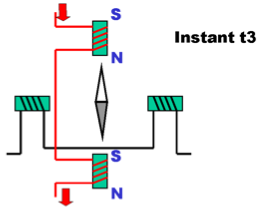
\includegraphics[width=0.9\textwidth]{images/moteur_paspas3}
    \caption{Instant $t_3$}
  \end{subfigure}
  \begin{subfigure}{.245\textwidth}
    \centering
    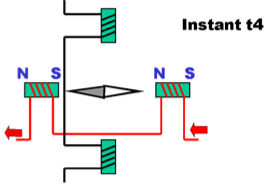
\includegraphics[width=0.9\textwidth]{images/moteur_paspas4}
    \caption{Instant $t_4$}
  \end{subfigure}
  \caption{Principe de fonctionnement d'un moteur pas à pas}
  \label{fig:paspas}
\end{figure}


\end{document}
